\chapter{动物在我们身边}\label{ch:g1:animals-around-us}

一只黑鸟在草坪上跳来跳去，一只猫在墙上看着它，
一只蚂蚁沿着门阶搬运一块比自己还大的面包屑。
\omterm{def:g1:animals-around-us:animal}{动物}就在我们身边——在花园里、在公园里、在房子里。
让我们像生物学家那样去观察它们：
看看它们的身体，也看看它们是怎样运动的。

\section{什么是动物？}

\begin{definition}[动物]\label{def:g1:animals-around-us:animal}
\emph{动物}\index{动物}是一种\omterm{def:g1:living-or-not:living}{生物}，它通过吃其他\omterm{def:g1:living-or-not:living}{生物}来取食——
这些\omterm{def:g1:living-or-not:living}{生物}可以是植物，也可以是其他动物——而且通常能够自己
四处移动。猫、黑鸟、鱼和蚂蚁都是动物。
我们人类也是动物。
\end{definition}

\begin{example}[一个花园里的动物]\label{ex:g1:animals-around-us:garden}
一个不大的花园里可以住着许多\omterm{def:g1:animals-around-us:animal}{动物}：一只黑鸟正从地里
拔出一条蚯蚓，蚯蚓本身，一只蜗牛趴在叶子上，
一只蜘蛛待在它的网里，一只蜜蜂停在花上，还有邻居家的猫。
无论大小，它们都会取食，也都会运动。
\end{example}

\begin{omfigure}
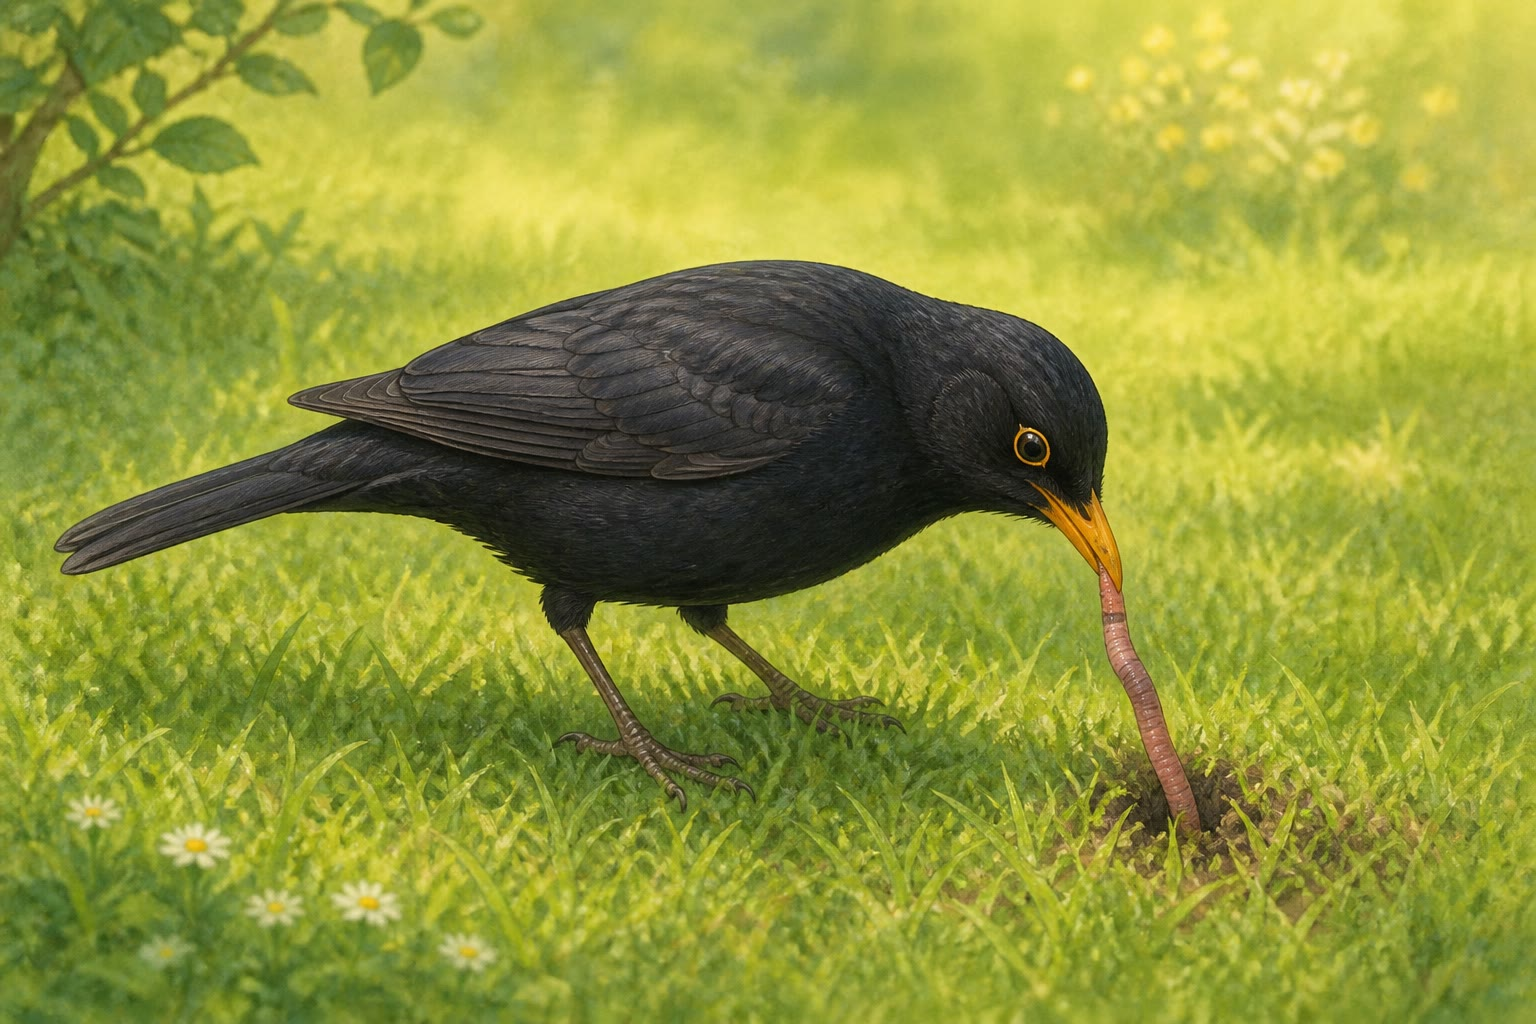
\includegraphics[width=0.62\linewidth]{images/book1/ai/g1-animals-blackbird.jpg}

{\small 花园里的忙碌景象：一只黑鸟正
从草坪上拔出它的早餐。}
\end{omfigure}

\begin{remark}[小不等于不重要]\label{rem:g1:animals-around-us:small}
蚂蚁和大象一样，都是\omterm{def:g1:animals-around-us:animal}{动物}。体型大小并不决定一个\omterm{def:g1:living-or-not:living}{生物}是不是\omterm{def:g1:animals-around-us:animal}{动物}：
关键看它能否取食和运动。
我们身边一些最神奇的\omterm{def:g1:animals-around-us:animal}{动物}，恰恰是最小的。
\end{remark}

\section{动物身体的各个部分}

\begin{definition}[身体的部分]\label{def:g1:animals-around-us:parts}
大多数\omterm{def:g1:animals-around-us:animal}{动物}都有\emph{头}\index{头}（头上有口和
大部分感觉器官）、身体，以及\emph{四肢}\index{四肢}——腿、
翅膀或鳍——它们用来运动。许多\omterm{def:g1:animals-around-us:animal}{动物}还有
\emph{尾巴}\index{尾巴}。
\end{definition}

\begin{omfigure}
\begin{tikzpicture}
  \node[anchor=south west, inner sep=0] (img) at (0,0)
    {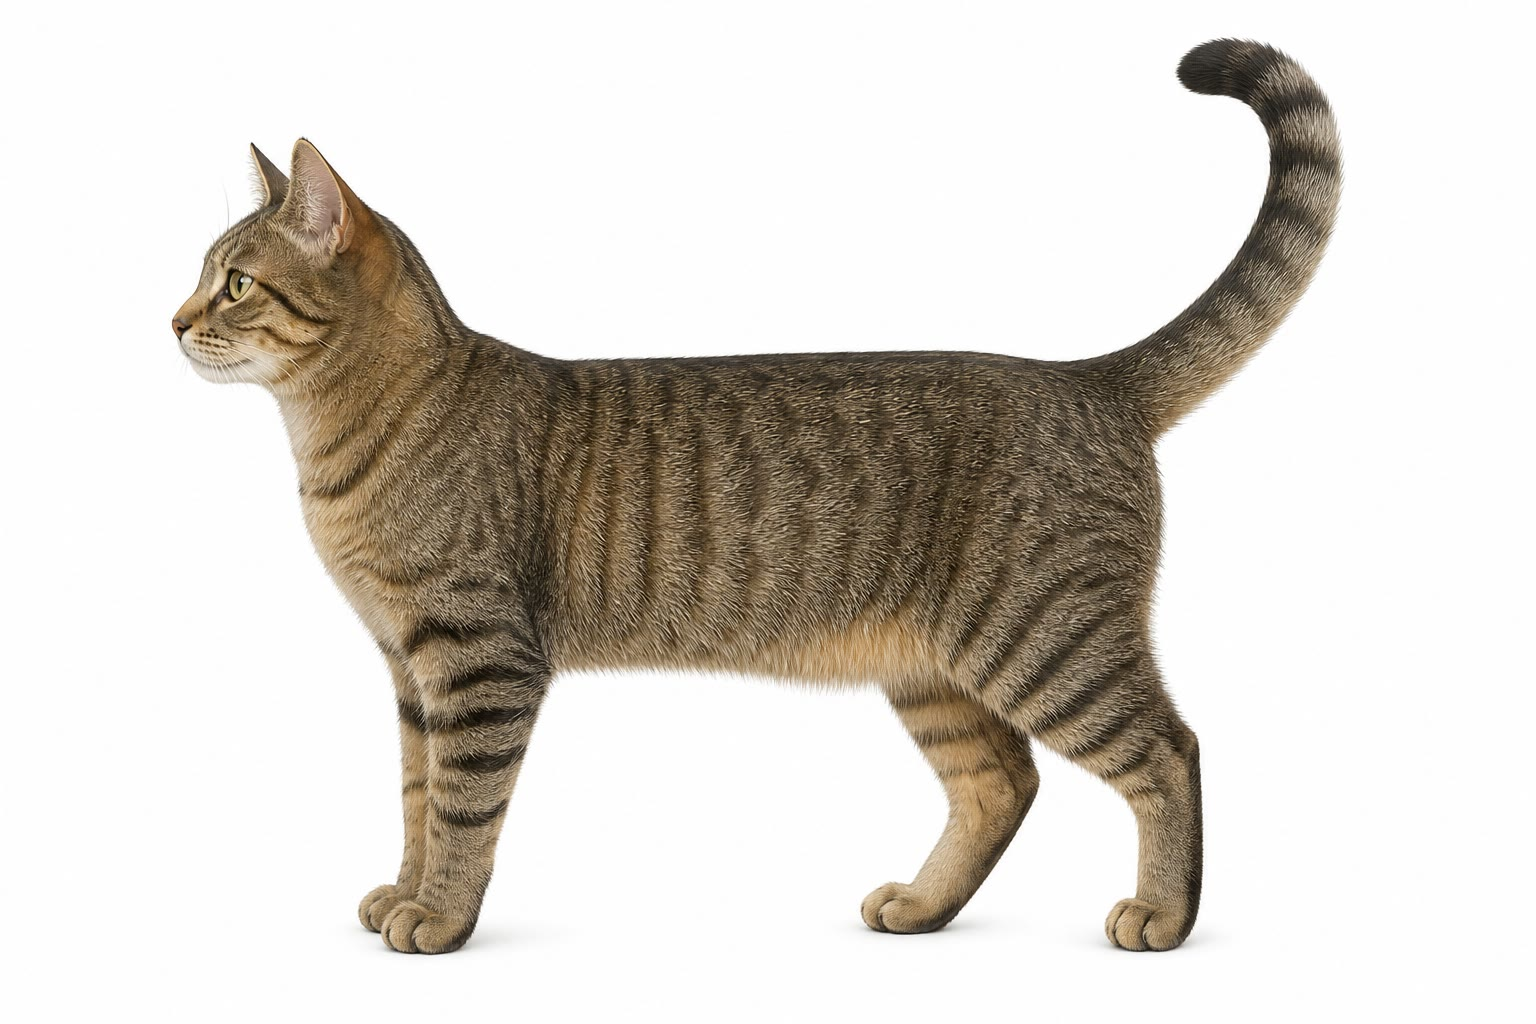
\includegraphics[width=0.6\linewidth]{images/book1/ai/fig-cat-side.jpg}};
  \begin{scope}[x={(img.south east)}, y={(img.north west)},
      every node/.style={font=\small}]
    \draw[omDef, thick] (0.17,0.80) -- (0.08,0.93) node[above] {头};
    \draw[omDef, thick] (0.55,0.64) -- (0.55,0.90) node[above] {身体};
    \draw[omDef, thick] (0.33,0.20) -- (0.30,-0.05) node[below] {腿（四肢）};
    \draw[omDef, thick] (0.84,0.84) -- (0.94,0.70) node[below] {尾巴};
  \end{scope}
\end{tikzpicture}

{\small 猫的身体各部分：头、身体、四条腿、尾巴。}
\end{omfigure}

\begin{example}[数一数腿]\label{ex:g1:animals-around-us:legs}
腿的数目很值得数一数。黑鸟用 $2$ 条腿走路，
猫有 $4$ 条腿，瓢虫有 $6$ 条腿，蜘蛛有 $8$ 条腿——
而蚯蚓和蜗牛根本没有腿，
可它们照样能到达想去的地方。
\end{example}

\begin{definition}[体表覆盖物]\label{def:g1:animals-around-us:covering}
\omterm{def:g1:animals-around-us:animal}{动物}的身体有覆盖物保护：
猫身上是\emph{皮毛}\index{皮毛}（毛发），黑鸟身上是\emph{羽毛}\index{羽毛}，
鱼身上是\emph{鳞片}\index{鳞片}，蜗牛身上是
\emph{壳}\index{壳}，
青蛙身上则是光滑湿润的\emph{皮肤}\index{皮肤}。
\end{definition}

\begin{example}[谁穿什么]\label{ex:g1:animals-around-us:covering}
摸一摸猫：是\omterm{def:g1:animals-around-us:covering}{皮毛}。捡起一根掉落的黑鸟\omterm{def:g1:animals-around-us:covering}{羽毛}：
又轻又软。仔细看看市场上的一条鱼：一排排闪亮的鳞片，
像一片片小小的屋瓦。三种\omterm{def:g1:animals-around-us:animal}{动物}，三种不同的“外衣”。
\end{example}

\section{动物如何运动}

\begin{proposition}[运动的方式]\label{prop:g1:animals-around-us:moving}
\omterm{def:g1:animals-around-us:animal}{动物}的运动方式与它们的肢体相适应：
\begin{itemize}
  \item 有腿的\omterm{def:g1:animals-around-us:animal}{动物}\emph{行走}、奔跑、跳跃或爬行——
        猫、草坪上的黑鸟和蚂蚁；
  \item 有翅膀的\omterm{def:g1:animals-around-us:animal}{动物}\emph{飞行}\index{飞行}——黑鸟、
        蜜蜂和蝴蝶；
  \item 有鳍的\omterm{def:g1:animals-around-us:animal}{动物}\emph{游动}\index{游动}——鱼；
  \item 没有肢体的\omterm{def:g1:animals-around-us:animal}{动物}滑行或蠕动——蜗牛用它那一只柔软的
        腹足滑行，蚯蚓则伸缩身体向前蠕动。
\end{itemize}
\end{proposition}
\admitted

\begin{omfigure}
\begin{tikzpicture}
  \draw[thick, omDef, fill=omDef!5] (0,0) rectangle (3.9,2.5);
  \draw[thick, omDef, fill=omDef!5] (4.3,0) rectangle (8.2,2.5);
  \draw[thick, omDef, fill=omDef!5] (8.6,0) rectangle (12.5,2.5);
  \node[font=\small\bfseries] at (1.95,2.15) {腿：行走};
  \node[font=\small\bfseries] at (6.25,2.15) {翅膀：飞行};
  \node[font=\small\bfseries] at (10.55,2.15) {鳍：游动};
  \node[font=\small, align=center, text width=3.6cm] at (1.95,1.0)
    {猫 \\ 蚂蚁 \\ 草坪上的黑鸟};
  \node[font=\small, align=center, text width=3.6cm] at (6.25,1.0)
    {蜜蜂 \\ 蝴蝶 \\ 空中的黑鸟};
  \node[font=\small, align=center, text width=3.6cm] at (10.55,1.0)
    {金鱼 \\ 鳟鱼 \\ 蝌蚪};
\end{tikzpicture}

{\small \omterm{def:g1:animals-around-us:parts}{四肢}与运动密不可分——而
黑鸟两次出现：腿用于草坪，翅膀用于空中。}
\end{omfigure}

\begin{remark}[一种动物，多种方式]\label{rem:g1:animals-around-us:several}
许多\omterm{def:g1:animals-around-us:animal}{动物}不止一种运动方式。黑鸟会走，
\emph{还}会飞；青蛙会游泳，\emph{还}会跳；鸭子会走，
会游泳，\emph{还}会飞。判断一种\omterm{def:g1:animals-around-us:animal}{动物}如何运动前，
先观察它一段时间。
\end{remark}

\begin{method}[观察动物]\label{met:g1:animals-around-us:observe}
要像生物学家那样描述一种\omterm{def:g1:animals-around-us:animal}{动物}：
\begin{enumerate}
  \item 观察各个部分：头、身体、\omterm{def:g1:animals-around-us:parts}{四肢}、尾巴；
  \item 数一数腿的条数，不要猜；
  \item 说出体表的覆盖物：\omterm{def:g1:animals-around-us:covering}{皮毛}、\omterm{def:g1:animals-around-us:covering}{羽毛}、鳞片、外壳、\omterm{def:g1:animals-around-us:covering}{皮肤}；
  \item 观察它如何运动：走、跳、飞、游、滑行；
  \item 说出你在哪里找到它：草坪、树上、池塘、石头下。
\end{enumerate}
不要伤害\omterm{def:g1:animals-around-us:animal}{动物}：观察之后，就让它继续前行。
\end{method}

\section{练习}

\begin{exercise}[$\star$]\label{exo:g1:animals-around-us:1}
说出图中猫身体的四个主要部分。
哪个部分长着眼睛和口腔？
\end{exercise}

\begin{exercise}[$\star$]\label{exo:g1:animals-around-us:2}
各有几条腿：(a) 母鸡？(b) 狗？(c) 瓢虫？(d) 蜘蛛？
(e) 蚯蚓？
\end{exercise}

\begin{exercise}[$\star$]\label{exo:g1:animals-around-us:3}
说出每种\omterm{def:g1:animals-around-us:animal}{动物}的覆盖物：绵羊、鸭子、鳟鱼、
蜗牛。
\end{exercise}

\begin{exercise}[$\star$]\label{exo:g1:animals-around-us:4}
本章中哪些\omterm{def:g1:animals-around-us:animal}{动物}会飞？它们都有什么
来代替前腿或手臂？
\end{exercise}

\begin{exercise}[$\star$]\label{exo:g1:animals-around-us:5}
蜗牛和蚯蚓没有腿。它们各自
如何运动？
\end{exercise}

\begin{exercise}[$\star$]\label{exo:g1:animals-around-us:6}
鸭子可以用三种方式运动。说出这三种方式，
并说明每种方式用到身体的哪个部分。
\end{exercise}

\begin{exercise}[$\star$]\label{exo:g1:animals-around-us:7}
根据\cref{def:g1:animals-around-us:animal}，蚂蚁为什么是\omterm{def:g1:animals-around-us:animal}{动物}？
请用该定义中的两个要点作答。
\end{exercise}

\begin{exercise}[$\star$]\label{exo:g1:animals-around-us:8}
试一试：到户外观察一种\omterm{def:g1:animals-around-us:animal}{动物}一小会儿——比如一只鸟、一只
昆虫或一只蜗牛。用
\cref{met:g1:animals-around-us:observe}中的五个步骤描述它。
\end{exercise}

\begin{exercise}[$\star\star$]\label{exo:g1:animals-around-us:9}
一位朋友说：“鱼类不可能是\omterm{def:g1:animals-around-us:animal}{动物}——它们不会走路！”
你会怎样回答？可以用\cref{prop:g1:animals-around-us:moving}。
\end{exercise}

\begin{exercise}[$\star\star$]\label{exo:g1:animals-around-us:10}
神秘\omterm{def:g1:animals-around-us:animal}{动物}：它有 $2$ 条腿、$2$ 只翅膀、\omterm{def:g1:animals-around-us:covering}{羽毛}，而且
不会飞，但跑得非常快。它是鸟吗？它会不会是
你所在街区跑得最快的\omterm{def:g1:animals-around-us:animal}{动物}？（想一想鸵鸟。）
\end{exercise}
